\paragraph{API Handling}

The \ac{API} handling is an essential part of the chatbot system, providing interaction between the frontend and the
backend. The \ac{API} connects various services, such as case management, message sending, and supplier handling, to
ensure that the system operates seamlessly. This section covers the most important functions from the \texttt{api.ts},
\texttt{v1.json}, and \texttt{v1.d.ts} files, which define the \ac{API}'s structure, types, and requests.

The \texttt{api.ts}
file defines core types and utilities that are crucial for \ac{API} interactions. It leverages TypeScript's type system
to define \ac{API} schema models, ensuring that all requests and responses are strongly typed and consistent throughout
the application.

The following snippet defines the types for \texttt{Case}, \texttt{State}, and \texttt{Message}, as shown in Code
\ref{lst:api-core-types}.

% @formatter:off
\begin{lstlisting}[language=JavaScript, caption={Core API Types (\texttt{api.ts})},
  firstnumber=1,label={lst:api-core-types}]
export type Case = components['schemas']['Case']
export type State = ArrayType<NonNullable<components['schemas']['Case']['state']>>
export type Message = components['schemas']['Message'] & {
  loading?: boolean
}
\end{lstlisting}
% @formatter:on

The \texttt{Case}, \texttt{State}, and \texttt{Message} types are derived from the OpenAPI schema (defined in the
\texttt{v1.json} file). These types ensure that every interaction with the \ac{API} adheres to the structure
defined by the backend. The \texttt{Message} type is extended to include a \texttt{loading} property
, allowing the frontend to track when a message is being processed, providing better feedback to the user.

The \texttt{v1.json} file represents the OpenAPI schema forthe backend. It defines all available \ac{API} endpoints,
their parameters, and their expected responses. This structure is crucial for understanding how the frontend interacts
with the backend.

Code \ref{lst:api-v1-json}, stored in \ref{subsec:frontend}, defines the \texttt{/api/v1/cases} endpoint for listing and
creating cases.

This endpoint supports both listing (GET) and creating (POST) cases. The GET method allows
filtering by \texttt{user\_id} and limiting the number of cases retrieved. The POST method requires a
\texttt{CreateCaseRequest} body to create a new case.
Each operation has a unique \texttt{operationId} (e.g., \texttt{list\_cases\_api\_v1\_cases\_get}), which is
used to reference and document the \ac{API} call.

Because OpenAPI is used, the \ac{API} Endpoints can be shown in the schema from Swagger as shown in Figure
\ref{fig:swaggerui}.

\begin{figure}[H]
  \centering
  \caption[Swagger UI]{Swagger UI \footnotemark}
  \label{fig:swaggerui}
  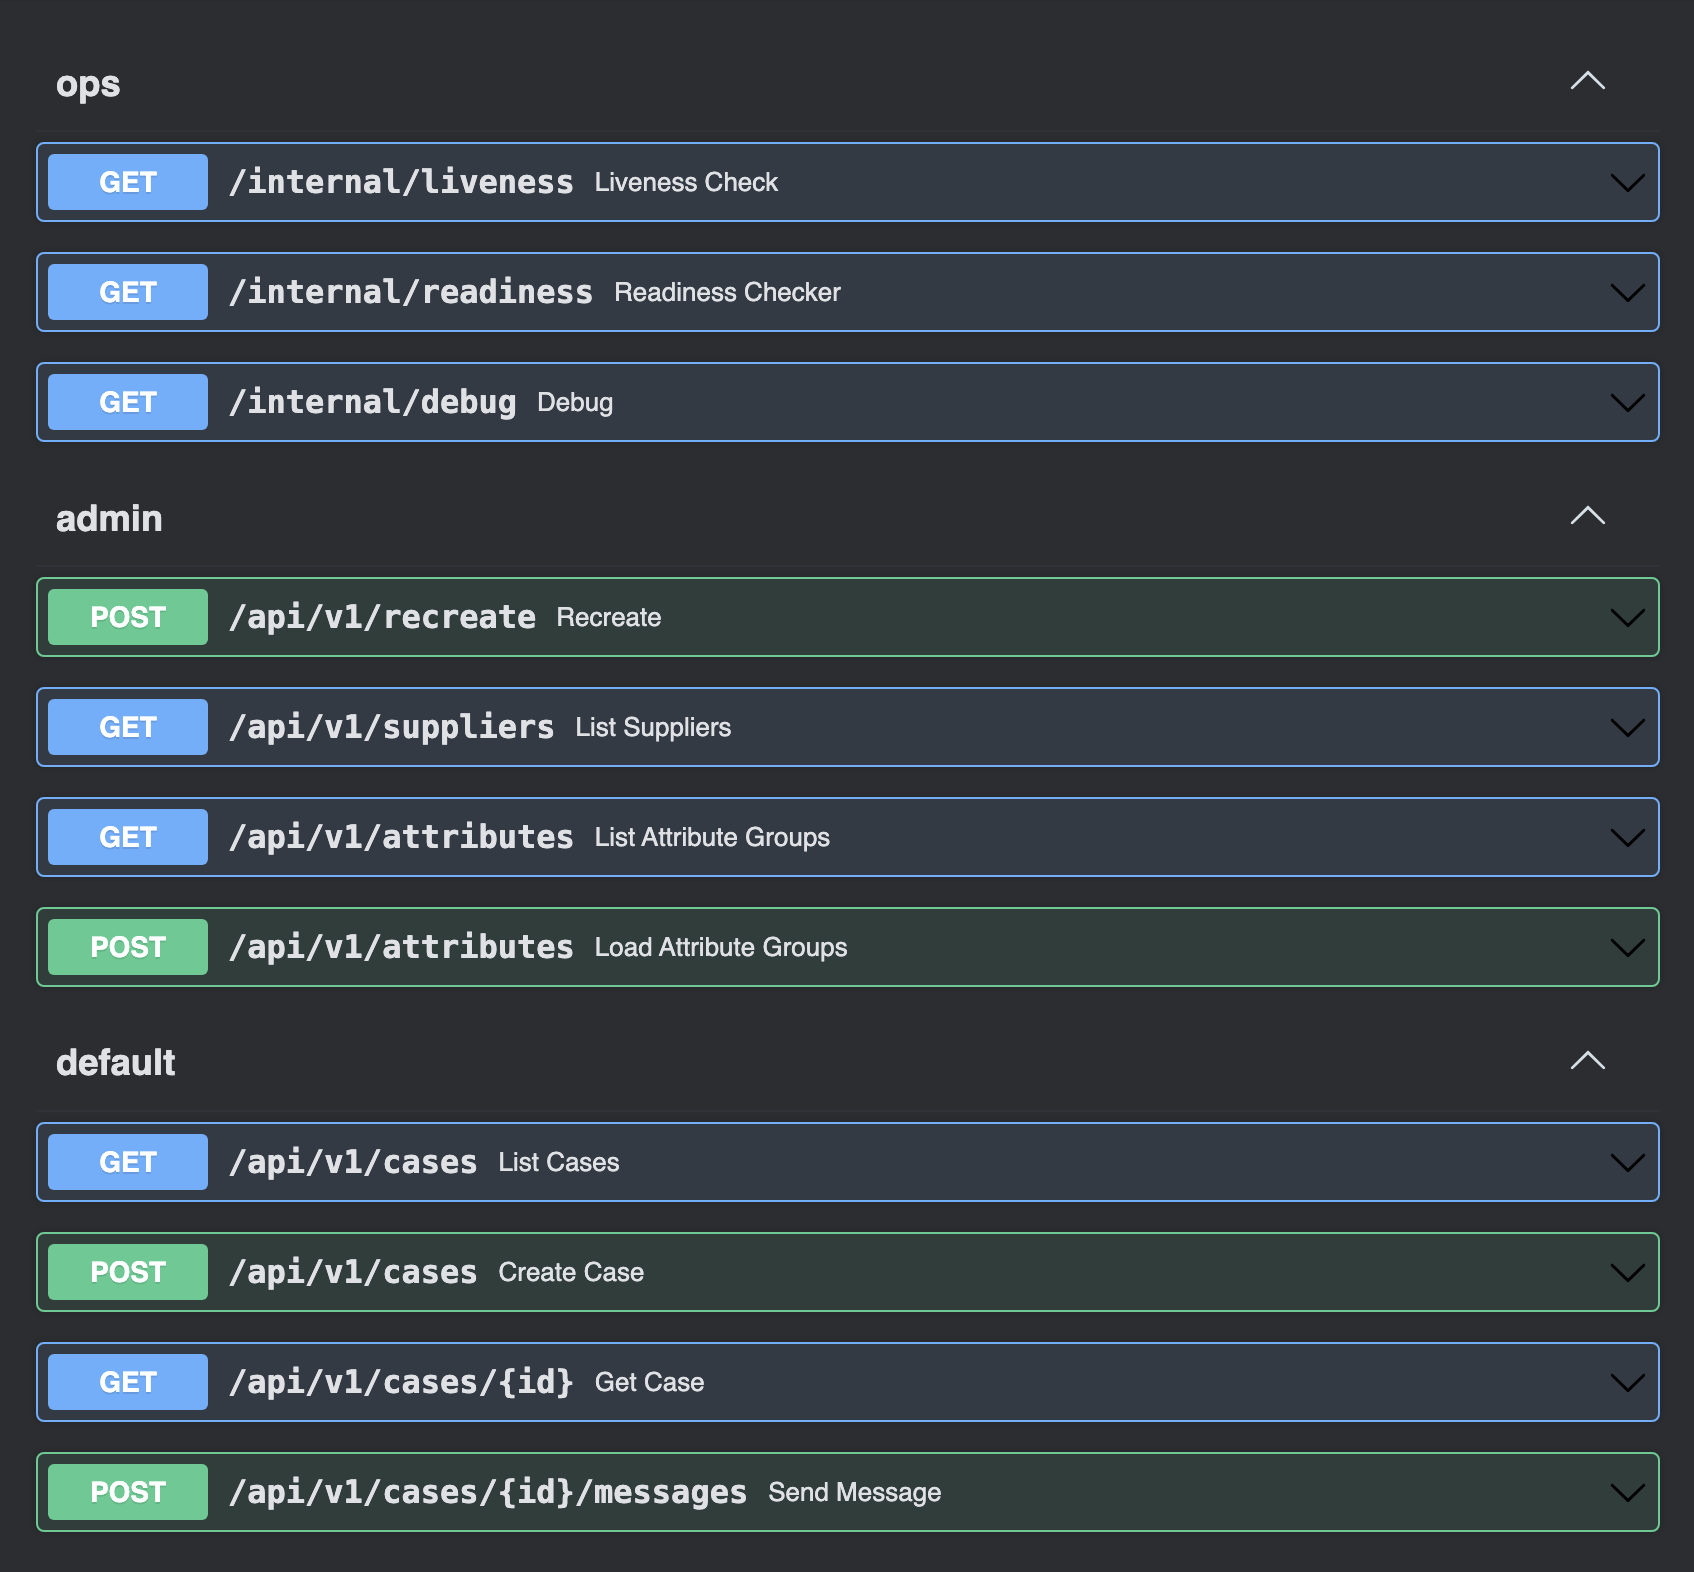
\includegraphics[width=1\textwidth]{abbildungen/Prototyping/Swagger_UI.png}
\end{figure}
\footnotetext{Own illustration}

This made it easy to test the \ac{API} Endpoints without implementing them directly in the code.

The \texttt{v1.d.ts} file defines the TypeScript types generated from
the OpenAPI schema, ensuring that all \ac{API} requests and
responses are typed correctly. This provides strong typing for all
interactions with the \ac{API}, helping prevent runtime errors and ensuring that the frontend and backend stay in sync.

The following snippet shows the type definition for the \texttt{Case} schema, as demonstrated in Code
\ref{lst:case-schema}.

% @formatter:off
\begin{lstlisting}[language=JavaScript, caption={Case Schema Definition (\texttt{v1.d.ts})},
  firstnumber=1,label={lst:case-schema}]
export interface components {
  schemas: {
    Case: {
      id: string;
      state?: components['schemas']['StateAttributeGroup'][];
      messages?: components['schemas']['Message'][];
      created_at: string;
      title?: string | null;
      case_type?: components['schemas']['SystemCaseTypeEnum'] | null;
    }
  }
}
\end{lstlisting}
% @formatter:on

This schema defines the structure of a \texttt{Case} object, which includes fields such as \texttt{id
}, \texttt{state}, \texttt{messages}, \texttt{created\_at}, and optional fields like \texttt{title} and \texttt{
case\_type}. The \texttt{state} field contains an array of \texttt{StateAttributeGroup} objects
, while the \texttt{messages} field contains an array of \texttt{Message} objects, demonstrating the
complexity of the data model.
